\documentclass[tikz,border=2pt]{standalone}
\usepackage{amsmath}
\usepackage{pgfplots}
\pgfplotsset{compat=1.18}

\begin{document}
% a_n -> +infinity: whatever bound M is chosen, from some index N on every term lies above M.
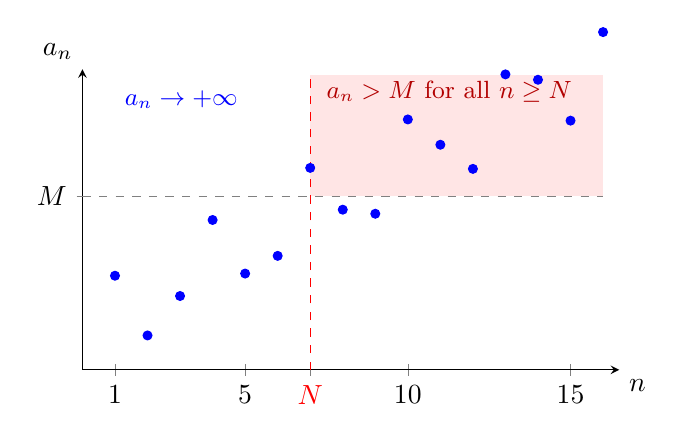
\begin{tikzpicture}
	\begin{axis}[
		axis lines=middle,
		xmin=0, xmax=16.5,
		ymin=0, ymax=5.2,
		xtick={1,5,10,15}, extra x ticks={7}, extra x tick labels={$N$}, extra x tick style={tick label style={red}},
		ytick={3}, yticklabels={$M$},
		xlabel={$n$}, ylabel={$a_n$},
		xlabel style={below right}, ylabel style={above left},
		clip=false,
		width=8.4cm, height=5.4cm
		]
		\fill[red!10] (axis cs:7,3) rectangle (axis cs:16,5.1);
		\addplot[gray, dashed, domain=0:16] {3};
		\draw[dashed, red] (axis cs:7,0) -- (axis cs:7,5.1);
		\addplot[only marks, mark=*, mark size=1.6pt, blue, samples at={1,...,16}] {0.3*x+0.8*sin(deg(2*x))+0.6};
		\node[red!70!black, anchor=south west, font=\small] at (axis cs:7.2,4.45) {$a_n>M$ for all $n\ge N$};
		\node[blue, anchor=north west, font=\small] at (axis cs:1,5.0) {$a_n\to+\infty$};
	\end{axis}
\end{tikzpicture}
\end{document}
